\documentclass[sigconf]{acmart}

\usepackage{amsmath}
\usepackage{amssymb}
\usepackage{amsthm}
\usepackage{geometry}
\usepackage{indentfirst}
\usepackage{graphicx}
\usepackage{multirow}
\usepackage{mathrsfs}
\usepackage{bbm}
\usepackage{cite}
\usepackage[linesnumbered,ruled]{algorithm2e}
\allowdisplaybreaks

\DeclareMathOperator*{\argmax}{arg\,max}

\newcommand{\sumi}{\sum\limits_i}
\newcommand{\sumj}{\sum\limits_j}
\newcommand{\sumk}{\sum\limits_k}
\newcommand{\sumij}{\sum\limits_{i,j}}

\newcommand{\sx}{x_{i,j}}
\newcommand{\sbp}{bp_{i,j}}

\newcommand{\sV}{V_{i,j}}
\newcommand{\sW}{W_{i,j}^{(k)}}
\newcommand{\sB}{B^{(k)}}

\newcommand{\sRPM}{RPM_{i,j}}

\newcommand{\salpha}{\alpha^{(k)}}
\newcommand{\stheta}{\theta^{(k)}}
\newcommand{\sbeta}{\beta_i}
\newcommand{\seta}{\eta_i}
\newcommand{\slambda}{\lambda_{i,j}}

\newcommand{\sF}{F_{i,j}}
\newcommand{\sS}{S_{i,j}}
\newcommand{\sG}{G_i}

\newcommand{\valpha}{\vec{\alpha}}
\newcommand{\vtheta}{\vec{\theta}}

\newcommand{\pprob}{\psi_1}
\newcommand{\pprice}{\psi_2}
\newcommand{\uff}{\mathscr{F}}
\newcommand{\uf}{f(bp; \pprob, \pprice, p(x))}

\newcommand{\dspresourceconstraint}{\sumij \sx \sW(\sbp) \le \sB}
\newcommand{\agapresourceconstraint}{\sumij \sx \sW(\sV) \le \sB}

\newcommand{\assignmentconstraint}{\sumj \sx \le 1}

\newcommand{\scoreconstraint}{\sbeta \ge \sS(\vec{\alpha})}

\newcommand{\linbp}{}
\newcommand{\ortbbp}{\sqrt{\frac{cRPM_i}{ROI}(1+\frac{1}{\lambda})+c^2}-c}
\newcommand{\dbbp}{\frac{\sRPM}{ROI}(1+\frac{1}{\alpha})}

\newcommand{\liniter}{bp_i^{'}=\frac{ROI_i(bp_i)}{ROI}bp_i}
\newcommand{\ortbiter}{\lambda^{'}=\frac{ROI}{ROI(\lambda)}\lambda}
\newcommand{\dbiter}{\alpha^{'} = \frac{ROI}{ROI(\alpha)}\alpha}

\newcommand{\mr}[2]{\multirow{#1}{*}{#2}}
\newcommand{\mc}[2]{\multicolumn{#1}{c|}{#2}}

\begin{document}

\title{Dual Based DSP Bidding Strategy and its Application}

\begin{abstract}
In recent years, RTB(Real Time Bidding) becomes a popular online advertisement trading method.
During the auction, each DSP is supposed to evaluate this opportunity and respond with an ad and corresponding bid price.
Generally speaking, this is a kind of assginment problem for DSP.
However, unlike traditional one, this assginment problem has bid price as additional variable.
It's essential to find an optimal ad selection and bid price determination strategy.
In this document, two major steps are taken to tackle it.
First, the augmented GAP(Generalized Assignment Problem) is proposed and a general bidding strategy is correspondingly provided.
Second, we show that DSP problem is a special case of the augmented GAP and the general bidding strategy applies.
To the best of our knowledge, our solution is the first DSP bidding framework
    that is derived from strict second price auction assumption
    and is generally applicable to the multiple ads scenario with various objectives and constraints.
Our strategy is verified through simulation and outperforms state-of-the-art strategies in real application.
\end{abstract}

\maketitle

\section{Introduction}

In recent years, RTB(Real Time Bidding) becomes a popular online advertisement trading method.
There are three major roles in the market, namely SSP(Supply Side Platform), DSP(Demand Side Platform), and AdX(Ad Exchange).
SSP controls huge amount of websites and earns money by supplying impressions.
DSP holds a lot of advertisers and makes profit through fullfilling their demands.
AdX, an online advertisement exchange, docks SSPs and DSPs and holds auctions.

In a typical scenario, an audience visits one of the SSP's websites, then the AdX is informed and an auction is initiated.
The AdX broadcasts bid request to DSPs and waits for a short time(e.g. 100ms).
Each DSP is supposed to evaluate this opportunity and respond with an ad and corresponding bid price.
The AdX gathers bid responses arriving before deadline and determines the winner and its cost.
Finally, the AdX notifies the SSP about the auction result and the SSP serves the winner's ad to the audience.

\begin{figure}[!h]
\centering
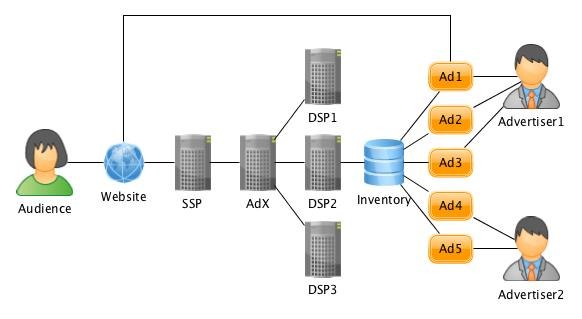
\includegraphics[width=1.0\linewidth]{./DSP.jpg}
\caption{Real Time Bidding}
\end{figure}

DSP usually provides two payment method for advertisers.
In PFI(Pay For Impression) mode, the advertiser sets RPM(Revenue Per Mili) and pays RPM for every 1000 impressions.
In PFU(Pay For Usage) mode, the advertiser sets commission rate and pays total bidding cost plus a fraction of it as commission.

Advertisers must set budgets for a certain period of time.
For performance consideration, both DSP and advertisers might set bounds for KPIs of interest.
DSP is supposed to distribute the bidding opportunities to ads in its inventory, maximizing its gain under above constraints.

For example, some DSPs are willing to maximize their profit under budget constraints in PFI mode,
    where profit is defined as the total revenue earned from advertisers minus total bidding cost payed to AdX.
Others prefer to maximize commission under both budget and average CPC(Cost Per Click) constraints in PFU mode,
    in which the total bidding cost divided by the total number of clicks must be within predefined threshold.

Generally speaking, this is a kind of assginment problem for DSP.
However, unlike traditional one, this assginment problem has bid price as additional variable.
It's essential to find an optimal ad selection and bid price determination strategy.
In this document, two major steps are taken to tackle it.
First, the augmented GAP(Generalized Assignment Problem) is proposed and a general bidding strategy is correspondingly provided.
Second, we show that DSP problem is a special case of the augmented GAP and the general bidding strategy applies.
To the best of our knowledge, our solution is the first DSP bidding framework
    that is derived from strict second price auction assumption and is generally applicable
    to the multiple ads scenario with various objectives and constraints.
These are the main contributions of this document.

%This document is organized as follows.
%In section 1, the background knowledge about RTB and DSP are introduced.
%In section 2, previous related works are described.
%In section 3, DSP problem is formalized as an mathematical optimization problem.
%In section 4, augmented GAP is studied with proof of its strong duality and resulting strategy.
%In section 5, the theory of augmented GAP is applied to DSP problem and two numeric optimization methods are discussed.
%In section 6, we verify our strategy through simulation.
%In section 7, we deploy our strategy in real application and experiment results are analyzed.
%In section 8, conclusions are drawn and future works are discussed.

\section{Related Work}

The linear bidding strategy proposed in \cite{M6D} is a heuristic method and,
    given base price, bids in propotion to the relative quality of impression.
\cite{WeinanZhang2014} suggests a non-linear relationship between optimal bid price and KPIs.
Based on calculus of variations, their strategy is derived from first price auction assumption.
Winning rate is explicitly modeled as a function of bid price, and,
    to find the analytical solution, this function must be of specific forms.
Both win rate and winning price are estimated in \cite{XiangLi2014}, and the corresponding bidding strategy is provided.
While all above researches consider only one campaign,
    \cite{WeinanZhang2015} extends \cite{WeinanZhang2014} to bidding strategy for multiple campaigns.
\cite{Joint2016} studies the joint optimization of multiple objectives with priorities.
\cite{Lift2016} argues that the bid price should be decided
    based on the performance lift rather than absolute performance value.
Risk management of RTB is discussed and risk-aware bidding strategy is proposed in \cite{Risk2017}.
By modeling the state transition via auction competition,
    the optimal bidding policy is derived in \cite{Reinforce2017} based on reinforcement learning theory.

The probability estimation of interested feedbacks plays a central role in performance based advertising.
CTR prediction is of great importance and extensively studied by researchers.
FTRL-Proximal, an online learning algorithm, is proposed in \cite{Google2013} and sparse model is learned for CTR prediction.
In \cite{Facebook2014}, a hybrid model which combines decision trees with logistic regression
    outperforms either of these methods on their own.
In \cite{FFM2016}, field-aware factorization machines are applied to predict CTR.
Compared with clicks, the conversions are even more rare and harder to predict.
To tackle the data sparseness, a hierarchical method is proposed in \cite{CVR} for CVR(Conversion Rate) prediction.
Feedbacks are usually delayed in practice and \cite{DelayedFeedback} tries to
    distinguish negative training samples without feedbacks eventually from those with delayed ones.

Bidding landscape is studied in \cite{YingCui2011} and log normal is used to model the distribution of winning price.
\cite{Wu2015} predicts win price with censored data, which utilizes both winning and losing samples in the sealed auction.
Traffic prediction for DSP is discussed in \cite{Traffic2016}.
Budget pacing is achieved through throttling in \cite{Throttle2015} and bid price adjustment in \cite{Pacing2013}.

Our work is mainly inspired by \cite{YeChen2011} in which compact allocation strategy,
    after modeling its problem as linear programming, is derived from complementary slackness.
Sealed second price auction is studied in \cite{SSPA1961}.
After all, DSP problem is a sort of online matching problem and \cite{Mehta} is an informative survey of this area.

\section{Formalization}

\subsection{Primal}

The DSP problem could be formalized as follows.
Once we bid $Impression$ with $Ad$, it results in gain $V$ and resource consumptions $W$, both of which are functions of $BidPrice$.
Our total gain should be maximized under resource constraints.
In addition, each $Impression$ should be distributed to no more than one $Ad$.
In this formalization, $B$ is set by either advertiser or DSP.
Family of $V$ and $W$ will be discussed shortly, while their parameter estimation is beyond the scope of this document.
To conquer the computational hardness, indicator variable $x$ is relaxed from $\{0, 1\}$ to $[0, 1]$.

\begin{alignat}{2}
    \max\limits_{\sx, \sbp} \quad & \sumij \sx \sV(\sbp) \quad    & {} \\
    \mbox{s.t.} \quad             & \dspresourceconstraint \quad  & \forall k \\
    \quad                         & \assignmentconstraint \quad   & \forall i \\
    \quad                         & \sx \ge 0 \quad               & \forall i,j
\end{alignat}

$i$ is the index of $Impression$

$j$ is the index of $Ad$

$k$ is the index of $Constraint$

$\sx$ is a relaxed variable, indicating whether $Impression_i$ should be given to $Ad_j$

$\sbp$, short for $BidPrice_{i,j}$, is a variable

$\sV(bp)$ is the gain function of $BidPrice$ with support $[0, \infty)$

$\sW(bp)$ is the $k$-th resource consumption function of $BidPrice$ with support $[0, \infty)$

$\sB$ is a resource limit constant

\subsection{Second Price Auction}

Most AdX adopts sealed second price auction mechanism.
The DSP with the highest bid price wins and pays the second highest bid price.
For example, three DSPs bid 2\$, 1\$, 3\$ respectively, so the third DSP wins and pays 2\$. 

Due to the dynamic nature of auction, the outcome is random.
To model this uncertainty, we define $p_i(x)$ as
   the distribution of the highest $BidPrice$ of all other DSPs for $Impression_i$ with support $[0, \infty)$.
Then we have $WinProb_i(bp)=\int_0^{bp} p_i(x) \mathrm{d} x$, and $WinPrice_i(bp)=\int_0^{bp} x p_i(x) \mathrm{d} x$.

It's worth to mention that we make little, if any, assumption about the form of $p_i(x)$.
In practice, $p_i(x)$ could be modeled either explicitly with method proposed by \cite{Wu2015} or inexplicitly when it's not mandatory.

\subsection{Utility Function Family}

The practical $V(bp)$ and $W(bp)$ in DSP problem come from a certain family
    which is defined here and whose properties are shown without proof.

\begin{definition}
$\uff = \{ \uf = \pprob WinProb(bp) + \pprice WinPrice(bp) = \int_0^{bp} (\pprob + \pprice x)p(x)dx \} $
\end{definition}

\begin{theorem}
$\uff$ is closed under linear combinations.
\end{theorem}

\begin{theorem}
Given $\forall f \in \uff$ with $\pprob > 0$ and $\pprice < 0$, we have $\argmax\limits_{bp} \uf = - \pprob / \pprice$.
\end{theorem}

\begin{theorem}
Given $\forall f,g \in \uff$ with common $p(x)$,
    we have $\frac{d^2h}{d^2g} = \frac{\pprob^g \pprice^h - \pprice^g \pprob^h}{(\pprob^g + \pprice^g bp)^3 p(bp)}$.
\end{theorem}

\subsection{Objectives}

There're three practical objectives in Table \ref{TableObjectives}.
In PFI mode, DSP could maximize either revenue(gross income) or profit(net income).
In PFU mode, DSP would maximize the commission. 

Taking maximizing profit in PFI mode for example, the profit is defined as $\sV(bp)=\sRPM{}WinProb_i(bp)-WinPrice_i(bp)$,
    and we have $\pprob=\sRPM$ and $\pprice=-1$.

\begin{table}
\caption{Practical Objectives\label{TableObjectives}}
\begin{center}
\begin{tabular}{|c|c|c|c|}
\hline
\mr{2}{Mode}   & \mr{2}{Type}       & \mc{2}{$\sV(bp)$} \\
\cline{3-4}
               &                    & $\pprob$   & $\pprice$ \\
\hline
\mr{2}{PFI}    & Revenue            & $\sRPM$    & 0 \\
\cline{2-4}
               & Profit             & $\sRPM$    & -1 \\
\hline
PFU            & Commission         & 0          & $Rate_j$ \\
\hline
\end{tabular}
\end{center}
\end{table}

\subsection{Constraints}

There're five practical constraints in Table \ref{TableConstraints}.
In PFI mode, DSP could set lower bound for ROI(Return on Investment).
In PFU mode, advertisers could set upper bound for CPS(Cost Per Show) and CPC.
In both modes, advertisers must set their budget.
Constraints like budget could be expressed in standard form naturally.
Others, though not so obvious at the first glance, could be rewritten into standard form as well.

Taking budget upper bound 2 in PFU mode for example, the budget consumption is defined as $\sV(bp)=WinPrice_i(bp)$,
    and we have $\pprob=0$ and $\pprice=1$ and the total consumption must not exceed $\sB=Budget^{(k)}$.

\begin{table}
\caption{Practical Constraints\label{TableConstraints}}
\begin{center}
\begin{tabular}{|c|c|c|c|c|}
\hline
\mr{2}{Mode} & \mr{2}{Type} & \mc{2}{$\sW(bp)$}                      & \mr{2}{$\sB$} \\
\cline{3-4}
             &              & $\pprob$              & $\pprice$      & \\
\hline
\mr{2}{PFI}  & Budget 1     & $\sRPM$               & 0              & $Budget^{(k)}$ \\
\cline{2-5}
             & ROI          & $-\sRPM$              & $ROI^{(k)}$    & 0 \\
\hline
\mr{3}{PFU}  & Budget 2     & 0                     & 1              & $Budget^{(k)}$ \\
\cline{2-5}
             & Average CPS  & $-CPS^{(k)}$          & 1              & 0 \\
\cline{2-5}
             & Average CPC  & $-CPC^{(k)}CTR_{i,j}$ & 1              & 0 \\
\hline
\end{tabular}
\end{center}
\end{table}

\section{Augmented GAP}

\subsection{Primal}

Now we propose the augmented GAP which extends the GAP in two ways.
First, user is subjected to multiple constraints and constraint is shared by multiple users.
Second, resource consumption becomes function of gain.
It's straightforward to see that DSP problem is a special case of augmented GAP.

\begin{alignat}{2}
    \max\limits_{\sx, \sV} \quad & \sumij \sx \sV \quad              & {} \\
    \mbox{s.t.} \quad            & \agapresourceconstraint \quad     & \forall k \\
    \quad                        & \assignmentconstraint \quad       & \forall i \\
    \quad                        & \sx \ge 0 \quad                   & \forall i,j
\end{alignat}

$i$ is the index of $Item$

$j$ is the index of $User$

$k$ is the index of $Constraint$

$\sx$ is a relaxed variable, indicating whether $Item_i$ should be given to $User_j$

$\sV$ is a gain variable

$\sW(V)$ is the $k$-th resource consumption function of $V$ with support $[0, \infty)$

$\sB$ is a resource limit constant

\subsection{Dual}

We define several basic functions and show the dual of augmented GAP based on them.
$\sF$ serves as sort of score function which evaluates the utility of distributing $Item_i$ to $User_j$.
The mathematical justification of $\sF$ will be given shortly, and it's worth to offer some intuitive explanations first.
Our gain $V$ is compromised by resource consumption $\sW(V)$ with so called opportunity cost,
    which could be calculated as unit $\sW(V)$ times price $\salpha$.

\begin{definition}
$\sF(V; \valpha) = V - \sumk \salpha \sW(V)$
\end{definition}

\begin{definition}
$\sV(\valpha) = \argmax\limits_V \sF(V; \valpha)$
\end{definition}

\begin{definition}
$\sS(\valpha) = \max\limits_V \sF(V; \valpha)$
\end{definition}

\begin{alignat}{2}
    \min\limits_{\salpha, \sbeta} \quad & \sumk \salpha \sB + \sumi \sbeta \quad   & {} \\
    \mbox{s.t.} \quad                   & \scoreconstraint \quad                   & \forall i,j \\
    \quad                               & \salpha \ge 0 \quad                      & \forall k \\
    \quad                               & \sbeta \ge 0 \quad                       & \forall i
\end{alignat}

\subsection{Strong Duality}

The strong duality of augmented GAP is provable under mild assumption.
A brief proof is provided here and more details are revealed in the appendix.

\begin{theorem}
If $W(V)$ is convex function of $V$, strong duality holds.
\end{theorem}

\begin{proof}
Several auxiliary problems are de€ned in Table \ref{TableAuxiliaryProblems}.
P is the primal and could be splited into 2 nested steps.
The inner step, given $\sx$, maximizes objective with $\sV$ as variables.
The outer step, maximizes objective with $\sx$ as variables.

\begin{table}
\caption{Auxiliary Problems\label{TableAuxiliaryProblems}}
\begin{center}
\begin{tabular}{|c|c|}
\hline
Name   & Description \\
\hline
P      & outer[inner] \\
\hline
D      & dualize(P) \\
\hline
DD     & dualize(dualize(P)) \\
\hline
d      & outer[dualize(inner)] \\
\hline
dd     & outer[dualize(dualize(inner))] \\
\hline
\end{tabular}
\end{center}
\end{table}

Since $W(V)$ is convex function of $V$, inner is a strong duality problem, inner = dualize(inner), P = d.
Since dualize(inner) is a strong duality problem, dualize(inner) = dualize(dualize(inner)), d = dd.
Since D is a strong duality problem, D = DD.
dd and DD happen to have the same form, dd = DD.
As a result, P = D, strong duality holds.
\end{proof}

\subsection{Dual Based Strategy}

With strong duality satisfied, several important properties are claimed about the optimal solution of both primal and dual problem,
    based on which we propose the dual based strategy.

\begin{theorem}
$\sV^* = \sV(\valpha^*)$.
\end{theorem}

\begin{theorem}
$\sx^*(\sbeta^* - \sS(\valpha^*)) = 0$.
\end{theorem}

\begin{corollary}
If $\sS(\valpha^*) < 0$, we have $\sx^* = 0$.
\end{corollary}

\begin{proof}
Since $\sS(\valpha^*) < 0$ and $\sbeta^* \ge 0$, we have $\sbeta^* > \sS(\valpha^*)$.
Now that $\sbeta^* - \sS(\valpha^*) > 0$ and $\sx^* \ge 0$,
    taking above theorem into consideration, $\sx^*$ must be 0,
    that is $Item_i$ should not be distributed to $User_j$.
\end{proof}

\begin{corollary}
If $S_{i,j_1}(\valpha^*) < S_{i,j_2}(\valpha^*)$, we have $x_{i,j_1}^* = 0$.
\end{corollary}

\begin{proof}
Similarly, since $S_{i,j_1}(\valpha^*) < S_{i,j_2}(\valpha^*)$ and $\sbeta^* \ge S_{i,j_2}(\valpha^*)$,
    we have $\sbeta^* > S_{i,j_1}(\valpha^*)$.
Now that $\sbeta^* - S_{i,j_1}(\valpha^*) > 0$ and $x_{i,j_1}^* \ge 0$, 
    taking above theorem into consideration, $x_{i,j_1}^*$ must be 0,
    that is $Item_i$ should not be distributed to dominated $User_{j_1}$.
\end{proof}

\begin{theorem}
$\sbeta^*(\sum\limits_j \sx^* - 1) = 0$.
\end{theorem}

\begin{corollary}
If $\exists j$ that $\sS(\valpha^*) > 0$, we have $\sum\limits_j \sx^* = 1$.
\end{corollary}

\begin{proof}
Since $\sS(\valpha^*) > 0$ and $\sbeta^* \ge \sS(\valpha^*)$, we have $\sbeta^* > 0$.
Now that $\sbeta^* > 0$ and $\sum\limits_j \sx^* - 1 \le 0$,
    taking above theorem into consideration, $\sum\limits_j \sx^*$ must be 1,
    which means $Item_i$ should not be discarded.
\end{proof}

In summary, for each $Item_i$, every $User_j$ should propose its own best score $\sS^*$ achieved by $\sV^*$.
$Item_i$ should be awarded to the dominating user if its best score is positive and discarded if that is negative.
Theoretically speaking, while most which are determined by above corollaries, behariors remain undefined in two special cases.
First, there might be multiple dominating users with the same best score.
Second, the best score of dominating user might be exactly zero.
In practice, however, both cases are probably rare due to the high resolution of items and users, and prone to cause relatively limited damage.
Ties could be broken by random or heuristics.

\begin{algorithm}
\caption{Dual Based Strategy for Augmented GAP}

\For{$Item_i \in \mathscr{I}$}
{
  \For{$User_j \in \mathscr{U}$}
  {
    $\sV^* = \sV(\valpha^*)$

    $\sS^* = \sS(\valpha^*)$
  }
  $j^* = \argmax\limits_j \sS^*$
  
  \If{$S_{i,j^*}^* \ge 0$} { bid with ($User_{j^*}$, $V_{i,j^*}^*$) }
}
\end{algorithm}

\section{Solution}

\subsection{Dual}

We define corresponding basic functions and show the dual of DSP problem based on them.
It's worth to notice that $\sF$ is linear combination of $\sV(bp)$ and $\sW(bp)$ from $\uff$
As a result, it must belong to $\uff$ too.

\begin{definition}
$\sF(bp; \valpha) = \sV(bp) - \sumk \salpha \sW(bp)$
\end{definition}

\begin{definition}
$\sbp(\valpha) = \argmax\limits_{bp} \sF(bp; \valpha)$
\end{definition}

\begin{definition}
$\sS(\valpha) = \max\limits_{bp} \sF(bp; \valpha)$
\end{definition}

\begin{alignat}{2}
    \min\limits_{\salpha, \sbeta} \quad & \sumk \salpha \sB + \sumi \sbeta \quad & {} \\
    \mbox{s.t.} \quad                   & \scoreconstraint \quad                 & \forall i,j \\
    \quad                               & \salpha \ge 0 \quad                    & \forall k \\
    \quad                               & \sbeta \ge 0 \quad                     & \forall i
\end{alignat}

\subsection{Strong Duality}

Given the nice property of $\uff$, it's easy to check that, in practical cases, $W(bp)$ is indeed convex function of $V(bp)$,
    which immediately justifies the strong duality of DSP problem.

\begin{theorem}
In practical cases, $W(bp)$ is convex function of $V(bp)$, strong duality holds
\end{theorem}

\subsection{Dual Based Strategy}

Here's corresponding dual based strategy for DSP problem.
Due to the nice property of $\uff$, $\sbp^*$ could be calculated easily without knowledge of $p_i(x)$.
In addition, ad is usually subjected to very limited number of constraints, which further reduces the complexity of this calculation.

In certain applications, $Q_{i,j}$ is the same for given $i$ and all $j$, then we have $j^* = \argmax\limits_j \sbp^*$.
For example, when maximizing profit under budget constraint in PFI mode,
    we have $\sF(bp) = \int_0^{bp} [(1-\salpha)\sRPM-x]p_i(x)dx$ and $Q_{i,j}$ is always 1.
By disposing of $p_i(x)$ completely from deciding process, it not only simplifies the computation,
    but also encourages $p_i(x)$ free training process.

\begin{algorithm}
\caption{Dual Based Strategy for DSP Problem}

\For{$Impression_i \in \mathscr{I}$}
{
  \For{$Ad_j \in \mathscr{A}$}
  {
    $\sF(bp; \valpha^*) = \int_0^{bp} (P_{i,j}-Q_{i,j}x)p_i(x)dx$

    $\sbp^* = \sbp(\valpha^*) = P_{i,j}/Q_{i,j}$

    $\sS^* = \sS(\valpha^*)$
  }
  $j^* = \argmax\limits_j \sS^*$
  
  \If{$S_{i,j^*}^* \ge 0$} { bid with ($Ad_{j^*}$, $bp_{i,j^*}^*$) }
}
\end{algorithm}

\subsection{Numeric Opmitization}

By fixing $\valpha$ in the dual problem, $\sbeta^*$ could be calculated independently,
    that is $\sbeta^* = \sbeta(\valpha) = \max \{ 0, \sS(\valpha) \forall j \}$.
It's easy to prove that $\frac{d\sbeta(\valpha)}{d\salpha}$ must be either $0$ or $-\sW(\sbp(\valpha))$.
Now we define $\sG(\valpha) = \sum\limits_k \frac{\salpha \sB}{N} + \sbeta(\valpha)$, in which $N$ is the number of impressions.
Then the dual problem could be rewritten as $\min\limits_{\valpha \ge 0} \sum\limits_i \sG(\valpha)$
    and solved by SGD(Stochastic Gradient Descent).
Due to the convexity of dual problem, it must converge to the global optimal $\valpha^*$.
This optimization method, though generally applicable, requires explicit modeling of $p_i(x)$.

Through executing our strategy in production environment, the randomized version of $\sW(\sbp(\valpha))$ is revealed
    and the gradients could be approximated with these feedbacks.
This optimization method is $p_i(x)$ free and much easier to implement.

\section{Simulation}

\subsection{Methodology}

To eliminate the uncertainty, our strategy is verified through simulation.
For simplicity, $p(x)$ is assumed to be a hill shaped distribution as depicted in Figure \ref{Hill} with its summit as the only parameter.
To mock the impressions, several pairs of $p(x)$ and $RPM$ are drawn randomly.
Three mocked ads are shown in Table \ref{TableMockedAds},
    based on which four simulated cases are proposed in Table \ref{TableSimulatedCases},
    three for single ad and one for multiple ads.

\begin{figure}[!h]
\centering
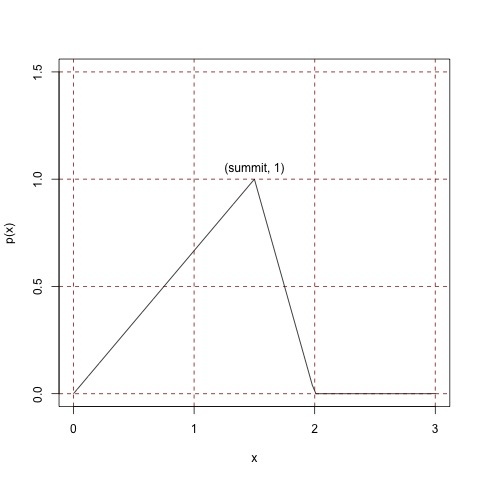
\includegraphics[width=0.5\linewidth]{./Hill.jpg}
\caption{Hill Shaped Distribution\label{Hill}}
\end{figure}

\begin{table}
\caption{Mocked Ads\label{TableMockedAds}}
\begin{center}
\begin{tabular}{|c|c|c|c|c|}
\hline
\mr{2}{Ad}     & \mr{2}{Mode}  & \mr{2}{Objective}  & \mc{2}{Constraint} \\
\cline{4-5}
               &               &                    & $k$   & Type \\
\hline
$Ad_1$         & PFI           & Profit             & 1     & Budget \\
\hline
$Ad_2$         & PFI           & Revenue            & 2     & ROI \\
\hline
\mr{2}{$Ad_3$} & \mr{2}{PFU}   & \mr{2}{Commission} & 3     & Budget \\
\cline{4-5}
               &               &                    & 4     & Average CPS \\
\hline
\end{tabular}
\end{center}
\end{table}

\begin{table}
\caption{Simulated Cases\label{TableSimulatedCases}}
\begin{center}
\begin{tabular}{|c|c|c|}
\hline
Case       & Inventory                          & \#Impressions \\
\hline
$Case_1$   & $\{Ad_1\}$                         & \mr{3}{5} \\
\cline{1-2}
$Case_2$   & $\{Ad_2\}$                         & \\
\cline{1-2}
$Case_3$   & $\{Ad_3\}$                         & \\
\hline
$Case_4$   & $\{Ad_j|j \in \{1,2,3\}\}$         & 15 \\
\hline
\end{tabular}
\end{center}
\end{table}

In $Case_1$, $Ad_1$ is in PFI mode with budget constraint, and DSP prefers to maximize its profit.
In $Case_2$, $Ad_2$ is in PFI mode with ROI constraint, and DSP prefers to maximize its revenue.
In $Case_3$, $Ad_3$ is in PFU mode with budget and average CPS constraint, and DSP prefers to maximize its commission.
$Case_4$ is a hybrid case with all above ads in the inventory.

Once the configurations are ready, cases are solved by SGD developed from our theory and brute force MC(Monte Carlo).
Due to the limited capacity of MC, only 5 impressions are generated for single ad cases and 15 for multiple ads case.

\subsection{Results and Analysis}

In all cases, constraints are satisfied by both SGD and MC, and objective values are shown in Table \ref{TableObjectiveValues}.
Both algorithms achieve similar primal objective values in the first three cases,
    while in the last one, however, MC must be far from convergence and is beaten by SGD.
In addition, the gap between primal and dual objective values proposed by SGD is negligible,
    as claimed by the strong duality theorem.

\begin{table}
\caption{Primal and Dual Objective Values\label{TableObjectiveValues}}
\begin{center}
\begin{tabular}{|c|c|c|c|}
\hline
\mr{2}{Case} & MC       & \mc{2}{SGD} \\
\cline{2-4}
             & Primal   & Primal   & Dual \\
\hline
$Case_1$     & 0.7423   & 0.7484   & 0.7484 \\
\hline
$Case_2$     & 3.4519   & 3.4719   & 3.4719 \\
\hline
$Case_3$     & 0.1000   & 0.1000   & 0.1006 \\
\hline
$Case_4$     & 10.7889  & 13.7849  & 13.7897 \\
\hline
\end{tabular}
\end{center}
\end{table}

Resource statistics and corresponding $\alpha$ of SGD are shown in Table \ref{TableResourcesAndAlpha}.
As mentioned earlier, the $\alpha$ serves as so called opportunity price of the resource.
Intuitively speaking, waste of resource with positive surplus shouldn't lead to any opportunity cost.
As a result, the corresponding $\alpha$ tends to be 0.

\begin{table}
\caption{Resources and $\valpha$\label{TableResourcesAndAlpha}}
\begin{center}
\begin{tabular}{|c|c|c|c|c|c|c|}
\hline
\mr{2}{Case}      & \mr{2}{Ad}     & \mc{4}{Resource}                                     & \mr{2}{$\alpha$} \\
\cline{3-6}
                  &                & $k$   & Limit       & Consumption     & Surplus      & \\
\hline
$Case_1$          & $Ad_1$         & 1     & 1.0000      & 1.0000          & 0.0000       & 0.6208 \\
\hline
$Case_2$          & $Ad_2$         & 2     & 0.0000      & 0.0000          & 0.0000       & 1.6369 \\
\hline
\mr{2}{$Case_3$}  & \mr{2}{$Ad_3$} & 3     & 1.0000      & 1.0000          & 0.0000       & 0.1001 \\
\cline{3-7}
                  &                & 4     & 0.0000      & -0.8120         & 0.8120       & 0.0008 \\
\hline
\mr{4}{$Case_4$}  & $Ad_1$         & 1     & 1.0000      & 0.9971          & 0.0029       & 0.3723 \\
\cline{2-7}
                  & $Ad_2$         & 2     & 0.0000      & -0.0004         & 0.0004       & 1.2480 \\
\cline{2-7}
                  & \mr{2}{$Ad_3$} & 3     & 1.0000      & 0.9981          & 0.0019       & 0.0929 \\
\cline{3-7}
                  &                & 4     & 0.0000      & -0.1089         & 0.1089       & 0.0273 \\
\hline
\end{tabular}
\end{center}
\end{table}

\section{Application}

\subsection{Scenario}

We also deploy our strategy in a real industrial application.
In our application, advertisers set budgets and pay for clicks, while DSP is willing to maximize revenue under global daily ROI constraint.
There're so many ads in our inventory that it's impossible to go through each ad before auction deadline.
Although these budgets are quite large totally, they are relatively small on average.

With a well calibrated RPM predictor, the problem could be transformed equivalently into one in PFI mode.
And to meet the latency requirement, the whole deciding process is decomposed into two stages with so called logical ad.
Logical ad should be seen as proxy of physical ads and binded with specific ad retrieval algorithm.
In the first stage, DSP is supposed to make decisions among just a few logical ads and respond in time.
In the second stage, once the chosen logical ad wins the auction, physical ad is lazily retrieved with corresponding algorithm.

\begin{figure}[!h]
\centering
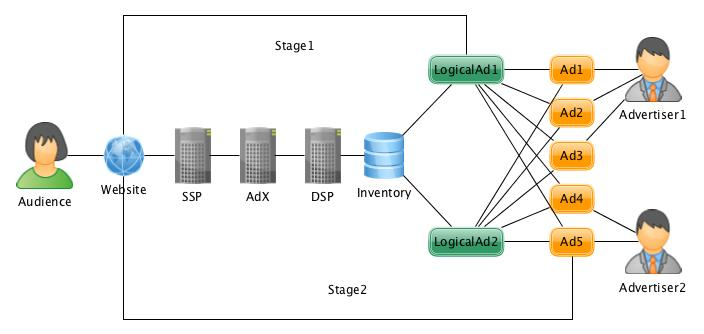
\includegraphics[width=1.0\linewidth]{./LogicalAd.jpg}
\caption{Real Time Bidding with Logical Ad}
\end{figure}

Our logical ads are actually based on four heterogeneous ad retrieval algorithms whose details are beyond the scope of this document.
These algorithms are sorted by their historical performance in descending orders and four logical ads are constructed correspondingly.

In summary, our problem could be approximately modeled as, given several logical ads with literally unlimited budget,
    maximizing revenue under global daily ROI constraint in PFI mode.
According to our theory, we have $\sF(bp) = \int_0^{bp} [(1+\alpha)\sRPM - \alpha{}ROIx]p_i(x)dx$ and $\sbp=\dbbp$.
Since there is only one resource constraint, superscript $k$ is omitted.
As $Q_{i,j}$ is always $\alpha{}ROI$, no $p_i(x)$ is required in deciding process.
To take full advantage of that, we adopt a simplified version of the $p_i(x)$ free optimization method, that is $\dbiter$.

\subsection{Experiment Groups}

We compare our strategy with a variation of linear bidding strategy.
In \cite{M6D}, it's suguested that $bp_i=\frac{CTR_i}{CTR}Bid$ with $Bid$ set by operation team.
In our application, it's natural to define $bp_i=\frac{ROI_i}{ROI}Bid$.
However, unlike $CTR_i$ which is independent of $bp_i$, $ROI_i$ actually varies with it.
Intuitively, we have $\liniter$.

We also apply optimal RTB theory to our application for comparison.
According to \cite{WeinanZhang2014}, we model the win probability as $w(bp;c)=\frac{bp}{c+bp}$ and bid with $bp_i=\ortbbp$,
    in which $c$ is fitted with historical data and $\lambda$ is iteratively tuned with $\ortbiter$.

Four experiment groups are shown in Table \ref{TableExperimentGroups}.
The first three groups are designed to compare different strategies with single logical ad,
    while the last group is used to test our strategy with multiple logical ads.

\begin{table*}
\caption{Experiment Groups\label{TableExperimentGroups}}
\begin{center}
\begin{tabular}{|c|c|c|c|c|c|}
\hline
Group    & Inventory                           & Strategy           & $\sbp$          & Iteration         & Period\\
\hline
$LIN$    & $\{LogicalAd_1\}$                   & Linear             & $bp_i$          & $\liniter$        & 24 hours \\
\hline
$ORTB$   & $\{LogicalAd_1\}$                   & Optimal RTB        & $\ortbbp$       & $\ortbiter$       & \mr{3}{10 minutes} \\
\cline{1-5}
$DB_{s}$ & $\{LogicalAd_1\}$                   & \mr{2}{Dual Based} & \mr{2}{$\dbbp$} & \mr{2}{$\dbiter$} & \\
\cline{1-2}
$DB_{m}$ & $\{LogicalAd_j|j \in \{1,2,3,4\}\}$ &                    &                 &                   & \\
\hline
\end{tabular}
\end{center}
\end{table*}

To eliminate potential bias, the experiment lasts for a whole ordinary week.
Bidding opportunities are distributed to each group randomly with equal probability.
For fairness, the same RPM predictor is shared by all groups.
The lower bound of global daily ROI is set to 3.5.

Parameters are periodically adjusted with performance data collected since last update.
The period is set to 24 hours for the $LIN$ group due to the data sparseness
    and 10 minutes as to the others for robustness and faster convergence.
Note that the more frequent update introduces inexplicitly a 10 minutes ROI constraint
    which is stricter than the daily one and might degenerate the theoratical optimal.

\subsection{Results and Analysis}

For each group, the daily statistics of four metrics are plotted in Figure \ref{Result},
    namely revenue, actual ROI, number of winning impressions and revenue per winning impression.

\begin{figure}[!h]
\centering
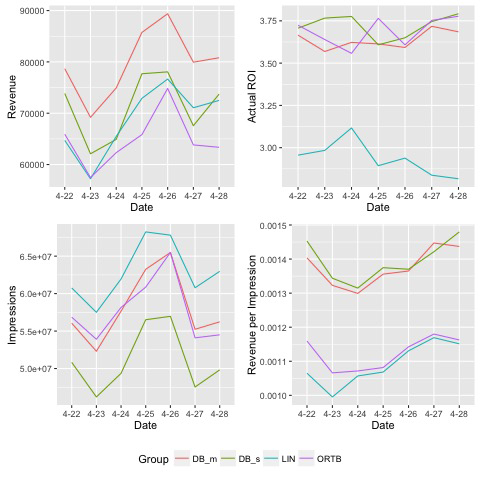
\includegraphics[width=1.0\linewidth]{./Result.jpg}
\caption{Experiment Results\label{Result}}
\end{figure}

The $LIN$, though with theoratical optimal intact, tends to earn less revenue than the others in practice.
In addition, it usually violates the global daily ROI constraint seriously, so it's an inferior strategy.

Compared with the $DB_s$ who claims a linear relationship between bid price and $RPM$,
    the $ORTB$, derived from first price auction assumption, suggests a non-linear one.
It is biased towards the impressions with low $RPM$ and against those with high $RPM$,
    which leads to more impressions and lower averaged quality.
While the daily ROI constraint is satisfied by both strategies,
    the $DB_s$ earns more revenue than the $ORTB$. As a result, the $DB_s$ is superior theoratically and practically.

The $DB_m$, as an ensemble of four ad retrieval algorithms,
    achieves the most revenue without violation of the daily ROI constraint and becomes the best strategy.

\section{Conclusions and Future Works}

In this document, we propose a dual based DSP bidding strategy
    derived from second price auction assumption according to convex optimization theory.
Our strategy is verified through simulation and outperforms state-of-the-art strategies in real application.
It's a theoratically solid and practically effective strategy with simple implementation and various applications.

Three problems remain unsolved and deserve further study.
First, is there a better way to solve $\valpha$ of large scale in dynamic environment?
On the one hand, in a typical DSP, there will be millions of constraints shared by similar number of ads.
Each of the constraints deserves a $\alpha$, which makes the vector $\valpha$ very large.
On the other hand, billions of impressions are broadcasted by AdX per day and bid by hundreds of DSPs simultaneously.
The bidding strategies are interactively adjusted by DSPs and the inventories are dynamically updated by advertisers,
    which makes the bidding landscape unstable.
Both properties make the optimal $\valpha$ relatively hard to solve.

Second, how to construct and index logical ads automatically in massive ads applications, balancing latency and performance?
It's obvious that both deciding and training processes share the same ad evaluation and maximum determination style,
    which makes their computational complexities linearly related with the number of candidate logical ads.
At one extreme, each ad is represented by exactly one logical ad, and the consequent latency is inacceptable.
At the other extreme, all ads are represented by the only logical ad, while the performance might be seriously degenerated.
A proper compromise combined with efficient indexing tricks will accelerate both processes by orders of magnitude.

Third, how to optimally break ties when they are common and critical in certain applications?
Taking an imaginary senario for example, all ads are in PFI mode with budget constraints, while DSP is willing to maximize its profit.
Besides, these ads share the universal constant RPM and are targeted respectively to sets of impressions which are overlaped.
In this circumstance, resolution of impressions and ads is extremely low and ties are very prevalent.

\appendix

\section{Strong Duality Proof}

Here we give the detailed proof of the strong duality. We first prove that P $\le$ D by dualizing P.

\begin{flalign*}
    P = & - \min\limits_{\substack{\sx,\sV \\ \agapresourceconstraint \\ \assignmentconstraint \\ \sx \ge 0 }} \{ - \sumij \sx \sV \} \\
      = & - \min\limits_{\sx,\sV} \{ \max\limits_{\salpha,\sbeta,\slambda \ge 0} \{ - \sumij \sx \sV \\
        & + \sumk \salpha [\sumij \sx \sW(\sV) - \sB] \\
        & + \sumi \sbeta (\sumj \sx - 1) + \sumij \slambda(-\sx) \} \} \\
      = & - \min\limits_{\sx,\sV} \{ \max\limits_{\salpha,\sbeta,\slambda \ge 0} \{ - \sumk \salpha \sB - \sumi \sbeta \\
        & + \sumij \sx [-\sV + \sumk \salpha \sW(\sV) + \sbeta - \slambda] \} \} \\
    \le & - \max\limits_{\salpha,\sbeta,\slambda \ge 0} \{ \min\limits_{\sx,\sV} \{ - \sumk \salpha \sB - \sumi \sbeta \\
        & + \sumij \sx [-\sV + \sumk \salpha \sW(\sV) + \sbeta - \slambda] \} \} \\
      = & - \max\limits_{\substack{ \salpha,\sbeta \ge 0 \\ \scoreconstraint }} \{ -\sumk \salpha \sB - \sumi \sbeta \} \\
      = & \min\limits_{\substack{ \salpha,\sbeta \ge 0 \\ \scoreconstraint }} \{ \sumk \salpha \sB + \sumi \sbeta \} \\
      = & D &&
\end{flalign*}

Next, we prove that D = DD by dualizing DD.

\begin{flalign*}
    D = & \min\limits_{\salpha,\sbeta} \{ \max\limits_{\sx,\stheta,\seta \ge 0 } \{ \sumk \salpha \sB + \sumi \sbeta \\
        & + \sumij \sx[\sS(\valpha) - \sbeta] \\
        & + \sumk \stheta (-\salpha) + \sumi \seta (-\sbeta) \} \} \\
      = & \min\limits_{\salpha,\sbeta} \{ \max\limits_{\sx,\stheta,\seta \ge 0 } \{ \sumk \salpha (\sB - \stheta) \\
        & + \sumi \sbeta (1 - \sumj \sx - \seta) + \sumij \sx \sS(\valpha) \} \} \\
      = & \max\limits_{\sx,\stheta,\seta \ge 0 } \{ \min\limits_{\salpha,\sbeta} \{ \sumk \salpha (\sB - \stheta) \\
        & + \sumi \sbeta (1 - \sumj \sx - \seta) + \sumij \sx \sS(\valpha) \} \} \\
      = & \max\limits_{\substack{\sx,\stheta \ge 0 \\ \assignmentconstraint }} \{ \min\limits_{\salpha} \{
          \sumk \salpha (\sB - \stheta) + \sumij \sx \sS(\valpha) \} \} \\
      = & DD &&
\end{flalign*}

After that, we prove that P = d by dualizing the inner step of P with the outer step unchanged.

\begin{flalign*}
    P = & \max\limits_{\substack{ \sx \ge 0 \\ \assignmentconstraint }} \{
          \max\limits_{\substack{ \sV \\ \agapresourceconstraint }} \{
          \sumij \sx \sV \} \} \\
      = & \max\limits_{\substack{ \sx \ge 0 \\ \assignmentconstraint }} \{
          - \min\limits_{\substack{ \sV \\ \agapresourceconstraint }} \{
          - \sumij \sx \sV \} \} \\
      = & \max\limits_{\substack{ \sx \ge 0 \\ \assignmentconstraint }} \{
          - \min\limits_{\sV} \{ \max\limits_{\salpha \ge 0} \{
          - \sumij \sx \sV \\
        & + \sumk \salpha [\sumij \sx \sW(\sV) - B^{(k)}] \} \} \} \\
      = & \max\limits_{\substack{ \sx \ge 0 \\ \assignmentconstraint }} \{
          - \min\limits_{\sV} \{ \max\limits_{\salpha \ge 0} \{ - \sumk \salpha B^{(k)} \\
        & + \sumij \sx [-\sV + \sumk \salpha \sW(\sV)] \} \} \} \\
      = & \max\limits_{\substack{ \sx \ge 0 \\ \assignmentconstraint }} \{
          - \max\limits_{\salpha \ge 0} \{ \min\limits_{\sV} \{ - \sumk \salpha B^{(k)} \\
        & + \sumij \sx [-\sV + \sumk \salpha \sW(\sV)] \} \} \} \\
      = & \max\limits_{\substack{ \sx \ge 0 \\ \assignmentconstraint }} \{
          - \max\limits_{\salpha \ge 0} \{ - \sumk \salpha \sB - \sumij \sx \sS(\valpha) \} \} \\
      = & \max\limits_{\substack{ \sx \ge 0 \\ \assignmentconstraint }} \{
          \min\limits_{\salpha \ge 0} \{ \sumk \salpha \sB + \sumij \sx \sS(\valpha) \} \} \\
      = & d &&
\end{flalign*}

At last, we prove that d = dd by dualizing the inner step of d with the outer step unchanged.

\begin{flalign*}
    d = & \max\limits_{\substack{ \sx \ge 0 \\ \assignmentconstraint }} \{
          \min\limits_{\salpha} \{ \max\limits_{\stheta \ge 0} \{
          \sumk \salpha \sB + \sumij \sx \sS(\valpha) \\
        & + \sumk \stheta (-\salpha)\} \} \} \\
      = & \max\limits_{\substack{ \sx \ge 0 \\ \assignmentconstraint }} \{
          \min\limits_{\salpha} \{ \max\limits_{\stheta \ge 0} \{
          \sumk \salpha (\sB - \stheta) + \sumij \sx \sS(\valpha) \} \} \} \\
      = & \max\limits_{\substack{ \sx \ge 0 \\ \assignmentconstraint }} \{
          \max\limits_{\stheta \ge 0} \{ \min\limits_{\salpha} \{
          \sumk \salpha (\sB - \stheta) + \sumij \sx \sS(\valpha) \} \} \} \\
      = & \max\limits_{\substack{ \sx,\stheta \ge 0 \\ \assignmentconstraint }} \{
          \min\limits_{\salpha} \{
          \sumk \salpha (\sB - \stheta) + \sumij \sx \sS(\valpha) \} \} \\
      = & dd &&
\end{flalign*}

It's obvious that DD and dd are of the same form, so DD = dd. As a result, we have P = D and strong duality holds.

\bibliographystyle{plain}
\bibliography{DSP}

\end{document}
